\documentclass[sigconf]{acmart}

\usepackage{booktabs}

\usepackage[utf8]{inputenc}
% Copyright
\setcopyright{none}
\editor{Alexander Acosta}
\editor{Julián Arango}
\settopmatter{printacmref=false}
\makeatletter
\def\@copyrightspace{\relax}
\makeatother

\settopmatter{printacmref=false}
\renewcommand\footnotetextcopyrightpermission[1]{}
\pagestyle{plain}

\begin{document}
\title{Clústering de Documentos a partir de Métricas de Similitud}
\subtitle{Big Data}

\author{Alexander Acosta Jiménez}
\affiliation{%
  \institution{Universidad EAFIT}
  \city{Medellín}
  \state{Colombia}
}
\email{aacosta8@eafit.edu.co}

\author{Julián David Arango López}
\affiliation{%
  \institution{Universidad EAFIT}
  \city{Medellín}
  \state{Colombia}
}
\email{jarangol@eafit.edu.co}


\begin{abstract}
El análisis de datos es un problema que ha sido estudiado por diversos campos,
actualmente este campo es abarcado principalmente por ciencias de la computación
y estadística debido al gran volumen de información y a la popularización del
uso del computador para almacenar información.

El manejo de un gran volumen de información requiere una adecuada infraestructura
y uso de recursos, en esta aproximación se busca aplicar herramientas
especializadas en el manejo de datos de gran volumen y algoritmos complejos,
en el análisis de datos, específicamente en el agrupamiento (clústering)
de documentos, utilizando  el algoritmo de machine learning K-means,
se implementa una solución no interactiva en Python 2.7, que utiliza la
arquitectura brindada por el framework Spark, para ser ejecutada en un ecosistema
Hadoop.

Como se resultado se comparan las implementaciones y los resultados obtenidos
entre HPC y Big data, utilizando datasets de ejemplo como Gutenberg.
\end{abstract}

\begin{CCSXML}
<ccs2012>
<concept>
<concept_id>10002944.10011123.10010916</concept_id>
<concept_desc>General and reference~Measurement</concept_desc>
<concept_significance>500</concept_significance>
</concept>
<concept>
<concept_id>10002944.10011123.10010912</concept_id>
<concept_desc>General and reference~Empirical studies</concept_desc>
<concept_significance>300</concept_significance>
</concept>
<concept>
<concept_id>10010147.10010169</concept_id>
<concept_desc>Computing methodologies~Parallel computing methodologies</concept_desc>
<concept_significance>500</concept_significance>
</concept>
</ccs2012>
\end{CCSXML}

\ccsdesc[500]{General and reference~Measurement}
\ccsdesc[300]{General and reference~Empirical studies}
\ccsdesc[500]{Computing methodologies~Parallel computing methodologies}

\keywords{Big Data, Distributed Computing,
  K-means, Intensive Computation, Intensive Data, Machine Learning,
    Data Mining, Clustering}
\maketitle

\section{Introducción}
K-means es un método de agrupamiento de datos utilizado en minería de datos.
Puede ser usado tanto en el campo científico como en el comercial, permite
buscar similaridades, entre las determinadas características representadas
con métricas, que posee un conjunto de datos o documentos.

El agrupamiento de datos es un problema NP-hard, es decir que normalmente el
problema requiere una cantidad apreciable de recursos computacionales para lograr
su ejecución y llegar una respuesta o solución, existen heuristicas que permiten
hallar una solución en tiempo razonable, el algoritmo k-means puede encontrar grupos de una
extención espacial comparable


Se implementó una solución que utiliza bibliotecas aportadas por el framework
de computación distribuida Apache Spark[2]
\footnote{Sitio oficial \url{https://spark.apache.org/}},
para el caso de Python se cuenta con Pyskpark[3], este modulo cuenta con la
biblioteca MLlib[4], que posee funcionalidades específicas de Spark[2]
para el campo de Machine Learning, entre ellas cuenta con los
métodos Term Frequency(TF) e Inverse Term Frequency (IDF), que permiten
obtener métricas de comparación entre los documentos para su posterior
agrupamiento con k-means, también incluido en MLlib como KMeans.

Se presenta una comparación entre la aproximación hallada para arquitecturas HPC
vs la solución para ambientes de Big Data, la colección de documentos ulizada
es un pequeño subconjunto[5]
\footnote{\url{https://web.eecs.umich.edu/~lahiri/gutenberg_dataset.html}}
del dataset Gutenberg [6] \footnote{\url{http://www.gutenberg.org/}}.

\section{Marco Teórico}
El agrupamiento de documentos es un problema que requiere de técnicas especiales
que permitan dar una solución óptima de agrupamiento, además de esto se requieren
suficientes recursos computacionales debido a la gran cantidad de documentos
que pueden llegar a ser analizados, además para que la solución sea generada
en un tiempo razonable.

Uno de los principales retos es la construcción de un algoritmo que permita
establecer la similitud entre documentos, ya que se debe de tener un criterio
de comparación, otro reto es agrupar cada uno de los documentos dependiendo
de su grado de similaridad en k conjuntos,

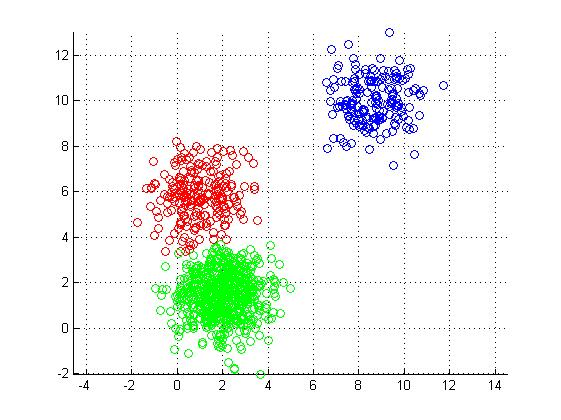
\includegraphics[scale=0.4]{datos}

Para agrupar los documentos  se ha utilizado un algoritmo K-means implementado
y adecuado específicamente para este tipo de arquitectura y es incluido dentro de la
biblioteca MLlib[4] que provee el framework Apache Spark [2].


\section{Análisis y Diseño}

\subsection{Caracterización de los documetos}
Los documentos contienen inicialmente palabras, y sólo con esto es imposible
calcular la similaridad que tienen entre sí, es necesario realizar una
cuantificación de las caracteristicas o atributos que posee cada documento para
que sea posible la comparación entre documentos.

\subsubsection{Term Frequency (TF)}
Para llevar a cabo la cuantificación, se ha utilizado el método ITF-IDF, que nos
provee una ponderación de terminos, muy importante para conocer además los
términos más relevantes en cada documento, TF nos brinda la frecuencia relativa,
es decir apariciones de cada palabra Wi en el documento Di.

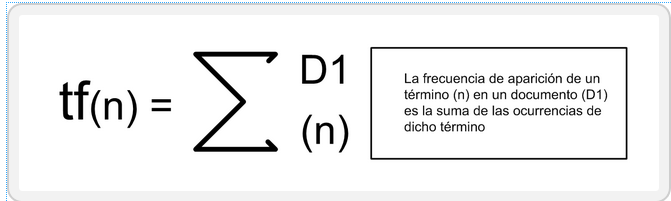
\includegraphics[scale=0.3]{tf_calculation}
\footnote{Tomado de [7]
\url{http://ccdoc-tecnicasrecuperacioninformacion.blogspot.com.co/2012/11/frecuencias-y-pesos-de-los-terminos-de.html}}


\subsubsection{Inverse Document Frequency (IDF)}
Es inversamente proporcional al número de documentos en los que aparece un
término ti, mientras menor la cantidad de documentos, y la frecuencia absoluta de
aparición de dicho termino, mayor será su IDF y viceversa.

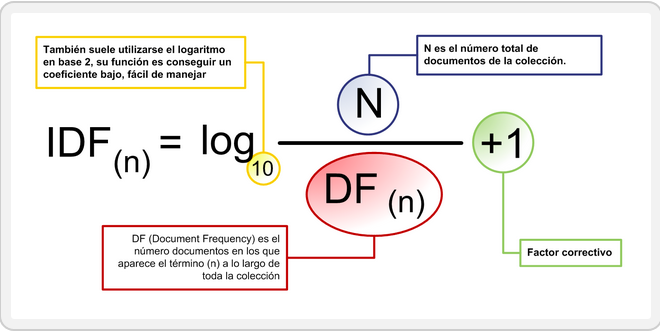
\includegraphics[scale=0.3]{idf_calculate}
\footnote{Tomado de [7]
\url{http://ccdoc-tecnicasrecuperacioninformacion.blogspot.com.co/2012/11/frecuencias-y-pesos-de-los-terminos-de.html}}


\subsubsection{Ponderación ITF-IDF}
Para calcular el peso de un término en un documento,se realiza el producto de su frecuencia de aparición en dicho documento (TF) y su frecuencia inversa de documento (IDF)
como se muestra a continuación.

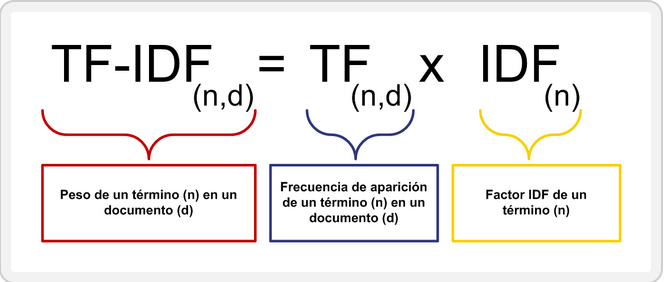
\includegraphics[scale=0.3]{tf-idf}
\footnote{Tomado de [7]
\url{http://ccdoc-tecnicasrecuperacioninformacion.blogspot.com.co/2012/11/frecuencias-y-pesos-de-los-terminos-de.html}}

\subsection{Algoritmo de agrupamiento}
\subsubsection{K-means}
Es un algoritmo de agrupamiento, cuyo objetivo es particionar un conjunto de n
elementos (en este caso documentos) en k subconjuntos los cuales contendrán
elementos similares entre sí, en cada iteración se calcula el promedio de
los elementos que pertenecen a un grupo en especifico, para así recalcular los centroides.
Como se mencionó anteriormente, se ha utilizado el algoritmo que provee MLlib[4]

\subsubsection{K-means}
Es un algoritmo de agrupamiento, cuyo objetivo es particionar un conjunto de n
elementos (en este caso documentos) en k subconjuntos los cuales contendrán
elementos similares entre sí, en cada iteración se calcula el promedio de
los elementos que pertenecen a un grupo en especifico, para así recalcular los centroides.

\subsection{Paralelización}
Mediante Hadoop File System (HDFS) [8], se carga el dataset, y se puede trabajar
sobre el dataset distribuido, el programa es repartido y ejecutado en varios nodos
por Spark, encargado del trabajo "sucio", se realizan operaciones a subconjuntos
del datase, y al añadir el procesamiento en memoria se optimiza notablemente
el rendimiento.

Posteriormente, se escribe la salida al sistema de archivos (HDFS) para obetener
la respuesta en los diferentes nodos de procesamiento.
\section{Implementación}
\subsection{Lectura de archivos}
Se implemento mediante el método wholeTextFiles que recibe como parámetro un directorio con documentos, y este método retorna una llave con el nombre del documento y valor que contiene el contenido del documento

\subsection{Cálculo de frecuencias}
Para el calculo de frecuencias se utilizó la biblioteca de spark TF-IDF
la cual se encarga de darle un peso a cada palabra de cada documento para así tener una matriz de frecuencias pero en vez de decir cuantas ocurrencias de una palabra hay en un documento, este algoritmo retorna la importancia de la
palabra en el documento.

Este algoritmo tiene 3 etapas. EL calculo de TF, el IDF y por último el TF-IDF que es el producto de los 2 anteriores cálculos.

\subsection{Asignación de centroides}
Luego de obtener esta "vectorización" de los términos ya podemos comparar
cuantitativamente cada uno de ellos, se procede a aplicar k-means.
El máster calcula los centroides iniciales aleatoriamente y los envía a todos los demás,
cada núcleo (worker) realiza la asignación de centroides para los documentos que le pertenecen
a partir de la minimización de la distancia desde cada documento a cada uno de
los centroides, se genera un diccionario con el índice del documento (key) y el
índice del centroide al que pertenece (value).

Como cada núcleo tiene solo una parte de los documentos, este diccionario es
enviado al máster para ser unificado y poder proceder con el recalculo de la
posición de los centroides.

\subsection{Cálculo de centroides}
Es aqui de donde el algoritmo toma su nombre, se calcula la nueva posición de cada
centroide como el promedio (mean) de todos los vectores (documentos) que pertenecen a
dicho centroide. El promedio se realiza dimensión por dimensión y el resultado
es un vector (nueva posición del centroide).

Este cálculo se ha paralelizado tambien. Se calcula el promedio de cada centroide
con los documentos que tiene cada núcleo/nodo, ya que cada uno de ellos es quien
tiene los vectores que se van a promediar y se guarda en un diccionario con el
índice del centroide (ki) como key y como valor el vector resultante del promedio
, este vector es multiplicado por la cantidad de documentos que se promediaron,
con el objetivo de calcular un promedio ponderado.
Este diccionario es enviado desde cada uno de los al máster, donde se calcula el
promedio ponderado, sumando los promedios parciales de cada centroide(k)
dimensión por dimensión y dividiendo esto por el total de documentos pertenecientes
a cada centroide, obteniendo así el promedio ponderado de los k centroides.

Nuevamente se envían estos valores a cada uno de los workers (slaves), para
proceder con una nueva iteración (si aplica) en donde se asignan centroides y
calculan promedios.

El método finaliza por número de iteraciones, que se pueden enviar como parámetro
o por defecto se puso un límite de 10.

Al final se imprime una respuesta indicando a que cluster pertenece cada documento.

 % Falta hablar de mover y el promedio ponderado
\section{Análisis de resultados}
Al realizar pruebas con el dataset de gutenberg se obtuvieron los siguientes resultados:
\begin{table}[htbp]
\begin{center}
\begin{tabular}{|l|l|}
\hline
Documentos & Tiempo\\
\hline \hline
50 & 63 s \\ \hline
100 & 65 s \\ \hline
150 & 74 s \\ \hline
200 & 80 s \\ \hline
250 & 92 s \\ \hline
350 & 100 s \\ \hline
400 & 107 s \\ \hline
\end{tabular}
\caption{Documentos de gutenberg.}
\label{tabla:sencilla}
\end{center}
\end{table}

En comparación a la ejecución serial ejecutada en un entorno de HPC, se puede observar que hay una mejoría exponencial de los tiempos, esto debido principalmente al uso de un ecosistema diseñado especialmente para un tipo de aplicaciones que requieren velocidad en el procesamiento, pero que además son ejecutadas con conjuntos grandes de datos, que en este caso son distribuidos y procesados paralelamente para un aumento del desempeño y disminución de tiempo de ejecución, como es mostrado en las cifras presentas.

\begin{table}[htbp]
\begin{center}
\begin{tabular}{|l|l|}
\hline
Documentos & Tiempo\\
\hline \hline
50 & 152.6 s \\ \hline
100 & 619.8 s \\ \hline
350 & 2976.9  s \\ \hline
\end{tabular}
\caption{Documentos de gutenberg(serial).}
\label{tabla:sencilla1}
\end{center}
\end{table}

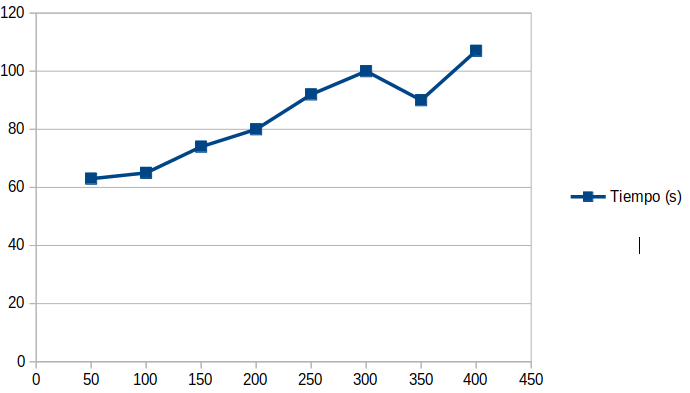
\includegraphics[scale=0.4]{tiempos}


%
% Para la ejecución se obtuvieron los siguientes resultados\footnote{Ejecución realizada
% teniendo en cuenta cada una de las palabras de todos los documentos.} :
% \begin{itemize}
%
%   \item   Con 20 documentos, tomo un tiempo de ejecucion de 3 minutos.
%   \item   Con 100 documentos, tomo un tiempo de ejecucion de 10 minutos.
%   \item   Con 300 documentos, tomo un tiempo de ejecucion de 50 minutos.
% \end{itemize}
%
% Para la ejecución en paralelo no seregistraron tiempos, debido a que no se notó
% una mejoría en los tiempos, estos ni siquiera eran razonables. Esto es debido a que
% se decidió trabajar con todas las palabras de los documentos, lo cual requiere una gran
% cantidad de tiempo para computar. Adicionalmente pasar esta gran cantidad de
% información a través de mensajes consume tiempo adicional. Pero se tiene en
% cuenta que el algoritmo fue ejecutado con pocos documentos para verificar su correcto
% funcionamiento.

\section{Conclusiones}
\begin{itemize}
\item Al utilizar un framework especializado en el procesamiento de datos masivos como lo es Spark [2], se evidencia un gran resultado en términos de tiempo de ejecución, porque esta diseñado especialmente para utilizar información distribuida, esto permite el uso de datasets de gran tamaño que dan respuestas en un tiempo muy corto.
\item El rendimiento en comparación del proyecto en serial y el paralelo orientado a BigData, se observaron unos mejores resultados en tiempo en el segundo (que utiliza Spark).
\end{itemize}

\section{Referencias}
\begin{enumerate}
\item [1] K-means: 2017. https://es.wikipedia.org/wiki/K-means. Accessed: 2017- 11- 23.
\item [2] Apache Spark™ - Lightning-Fast Cluster Computing: 2017. https://spark.apache.org/. Accessed: 2017- 11- 23.
\item [3] Welcome to Spark Python API Docs! — PySpark 2.2.0 documentation: 2017. http://spark.apache.org/docs/2.2.0/api/python/. Accessed: 2017- 11- 23.
\item [4] MLlib | Apache Spark: 2017. https://spark.apache.org/mllib/. Accessed: 2017- 11- 23.
\item [5] Gutenberg Dataset: 2017. \url{https://web.eecs.umich.edu/~lah/gutenberg_dataset.html}. Accessed: 2017- 10- 23.
\item [6] Project Gutenberg: 2017. http://www.gutenberg.org/. Accessed: 2017- 10- 23.
\item [7]Frecuencias y pesos de los términos de un documento: 2017. http://ccdoc-tecnicasrecuperacioninformacion.blogspot.com.co/2012/11/frecuencias-y-pesos-de-los-terminos-de.html. Accessed: 2017- 11- 23.
\item [8] Hadoop File System 2017. https://hadoop.apache.org/docs/stable/hadop-project-dist/hadoop-hdfs/HdfsUserGuide.html. Accessed: 2017- 11- 23.
\end{enumerate}

  % \bibliographystyle{ACM-Reference-Format}
  % \bibliography{sample-bibliography}
\end{document}
